\documentclass{beamer}

\usepackage[utf8]{inputenc}
\usepackage[english]{babel}
\usepackage{textpos}
\usepackage{graphicx}
\usepackage{textcomp}
\usepackage{animate}
\usepackage{comment}
%\usepackage{multicol}
%\setlength{\columnsep}{5cm}
\usepackage{amsmath}
\usepackage{verbatim}
\usepackage{varwidth}
\usepackage{caption}
\usepackage{dcolumn}
\usepackage{amssymb}
\usepackage{algorithm}
\usepackage{algorithmic}
%\usepackage{physics}
\usepackage{hyperref}
\usepackage{scalerel,stackengine}
\usepackage{fancyvrb}


\newcommand{\code}[1]{\texttt{#1}}
\newcommand{\shp}{$>>>$ }
\newcommand{\tab}{\hspace*{22pt}}

\usetheme{Madrid}

\title{Intro to Python}
\author{EEC 3150}
\date{}

\begin{comment}
\institute
{
	GTA, Computational Science\\
	Middle Tennessee State University
}
 
\date{COMS 7300, Spring 2016}
\end{comment}

%%%%%%%%% BEGIN DOCUMENT %%%%%%%%%
%%%%%%%%% BEGIN DOCUMENT %%%%%%%%%
%%%%%%%%% BEGIN DOCUMENT %%%%%%%%%

\begin{document}

% get title page 
\frame{\titlepage}
 
%%%%%%%%%%
%%%%%%%%%%
\begin{frame}	
	\frametitle{Outline}
	\tableofcontents	
\end{frame}


%%%%%%%%%%
%%%%%%%%%%
\section{Programming in General}

\begin{frame}	
	\center{\Huge{Programming in General}}
\end{frame}

\begin{frame}	
	\frametitle{Programming in General}
	
	\begin{alertblock}{Defn: ``computer programming''}
		\begin{itemize}
			\item \textbf{Computer programming} is the process of performing a given computational task by designing, building, and executing a computer program (Wikipedia).
			\item \textbf{Computer programs} are sequences of instructions (or commands, statements) that is written in a programming language and designed to complete some computational task
			\item A \textbf{programming language} is the language in which a computer program is written. It contains all of the common features of human languages: vocabulary (set of words), syntax/grammar (rules for constructing sequences of words), semantics (meaning). 
		\end{itemize}
	\end{alertblock}
	
\end{frame}

\begin{frame}	
	\frametitle{Programming in General}
	
	\begin{block}{Types of programming languages:}
		\begin{itemize}
			\item Procedural languages
			\item Object-oriented languages (OOP)
			\item Functional languages
			\item Visual languages
			\item Assembly languages
			\item Machine languages
			\item Hardware description languages
			\item Query languages
			\item Synchronous/Asynchronous languages
			\item Markup/typesetting languages
		\end{itemize}
		
		\vspace{8pt}
		
		Python is procedural, object-oriented, and synchronous
	\end{block}
	
\end{frame}

\begin{frame}	
	\frametitle{Programming in General}
	
	\begin{alertblock}{Defn: ``low-level'' vs. ``high-level''}
		\minipage{0.5\textwidth}
			Programming languages can be classified into several different categories:
			
			\vspace{10pt}
			
			\begin{itemize}
				\item 	\textbf{Low-level} languages deal with instructions and data objects which are at or near the level of machine code, i.e., individual bits.
				\item \textbf{High-level} languages deal with instructions and data objects which are at a more abstract, human-readable level.
			\end{itemize}
		\endminipage\hfill
		\minipage{0.5\textwidth}
			\begin{figure}[ht]
				\centering
				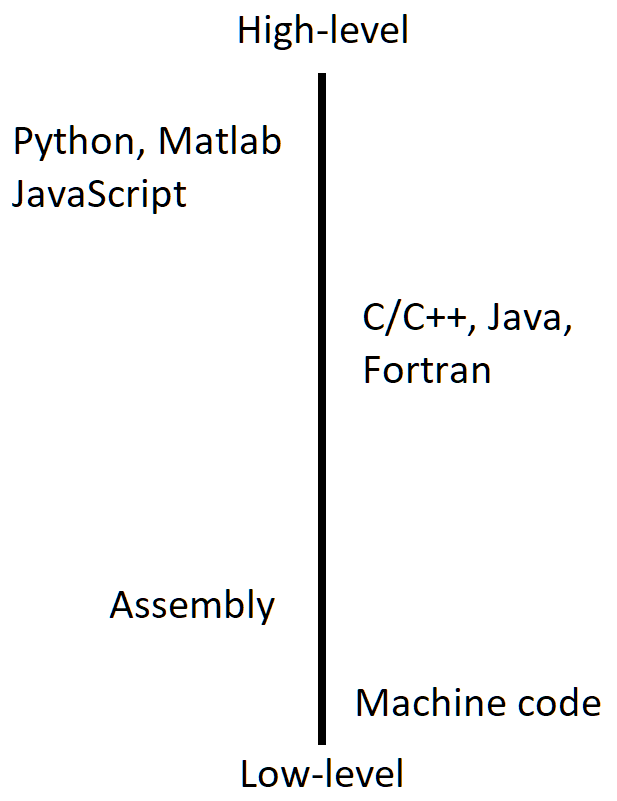
\includegraphics[width=0.8\linewidth]{LanguageLevels}
				\caption{Levels or progamming languages}
			\end{figure}
		\endminipage\hfill
		
		\vspace{-8pt}
		
	\end{alertblock}
	
\end{frame}

\begin{frame}	
	\frametitle{Programming in General}
	
	\begin{block}{Defn: ``low-level'' vs. ``high-level''}
		Low-level:
		\begin{itemize}
			\item Pros: execute faster, more control over under-the-hood aspects
			\item Cons: code is very precise but verbose/tedious, not as easily readable
		\end{itemize}
		
		\vspace{10pt}
		
		High-level:
		\begin{itemize}
			\item Pros: easier to write, complicated tasks can be written in fewer lines of code, under-the-hood stuff handled for you
			\item Cons: execute slower, less control
		\end{itemize}
		
		\vspace{10pt}
		
		Rule of thumb: execution speed and ease of reading/writing are typically inversely related
		
	\end{block}
	
\end{frame}

\begin{frame}	
	\frametitle{Programming in General}
	
	\begin{alertblock}{Defn: ``interpretted'' vs. ``compiled''}
		To run/execute your program, the computer must convert the code into low-level format that it understands:
		\begin{itemize}
			\item 	\textbf{Interpretted} languages (Python, Matlab, JavaScript) perform this conversion \textit{line-by-line}, as well as execute the program line-by-line.
			\item \textbf{Compiled} languages (C/C++, Java, Fortran) convert (i.e., compile) the \textit{entire} program at once, creating a new file that can be executed.
		\end{itemize}
		
		\vspace{10pt}

		Pros and Cons		:
		\begin{itemize}
			\item Compiled languages are MUCH faster, but must be recompiled whenever a change is made to the source code. The compiled program often cannot be run on another machine.
			\item Interpretted languages are usually high-level, making them easier to read/write. Also, their error messages can be easier to understand due to the line-by-line nature of the interpretter.
		\end{itemize}
		
	\end{alertblock}
	
\end{frame}

%%%%%%%%%%
%%%%%%%%%%
\section{About Python}

\begin{frame}	
	\center{\Huge{About Python}}
\end{frame}

\begin{frame}	
	\frametitle{About Python}
	
	\begin{block}{Counting backward from 10 in four progamming languages:}
		Do you find anything noteworthy about the Python code?

		\begin{figure}[ht]
			\centering
			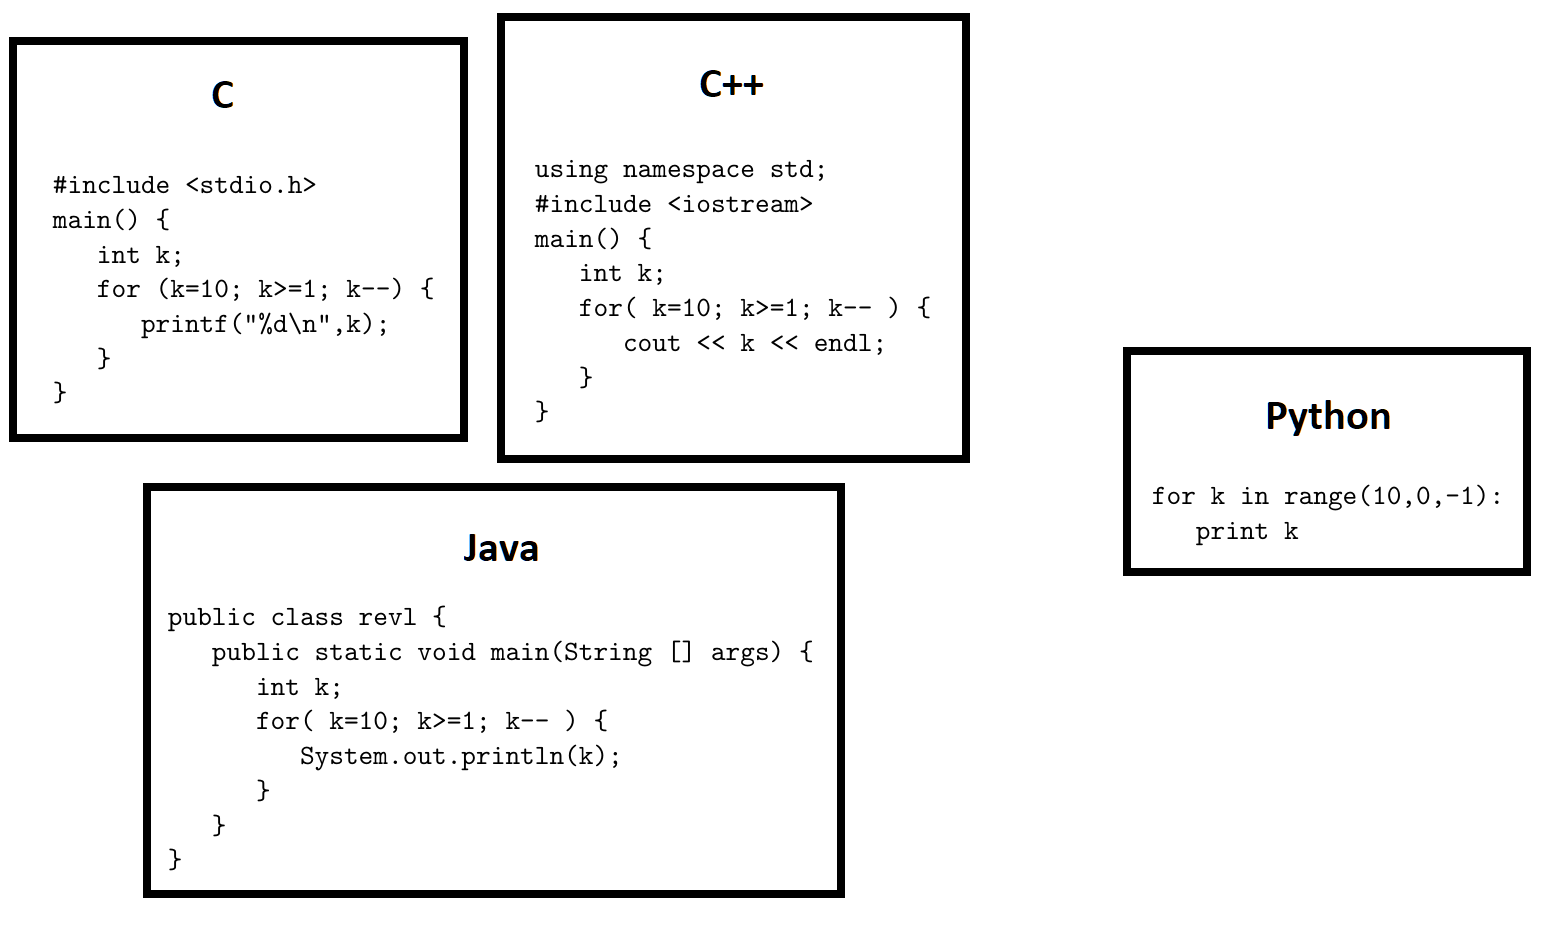
\includegraphics[width=0.8\linewidth]{SameLanguage}
			%\caption{Same program in 4 progamming languages}
		\end{figure}
		
	\end{block}
	
\end{frame}

\begin{frame}	
	\frametitle{About Python}
	
	\begin{block}{Counting backward from 10 in four progamming languages:}
		\minipage{0.4\textwidth}
			Python:
			\begin{itemize}
				\item Shorter than all the others
				\item No semisolons
				\item No curly braces (uses tabs instead)
				\item No need to declare variables before use
			\end{itemize}
		\endminipage\hfill
		\minipage{0.6\textwidth}
			\begin{figure}[ht]
				\centering
				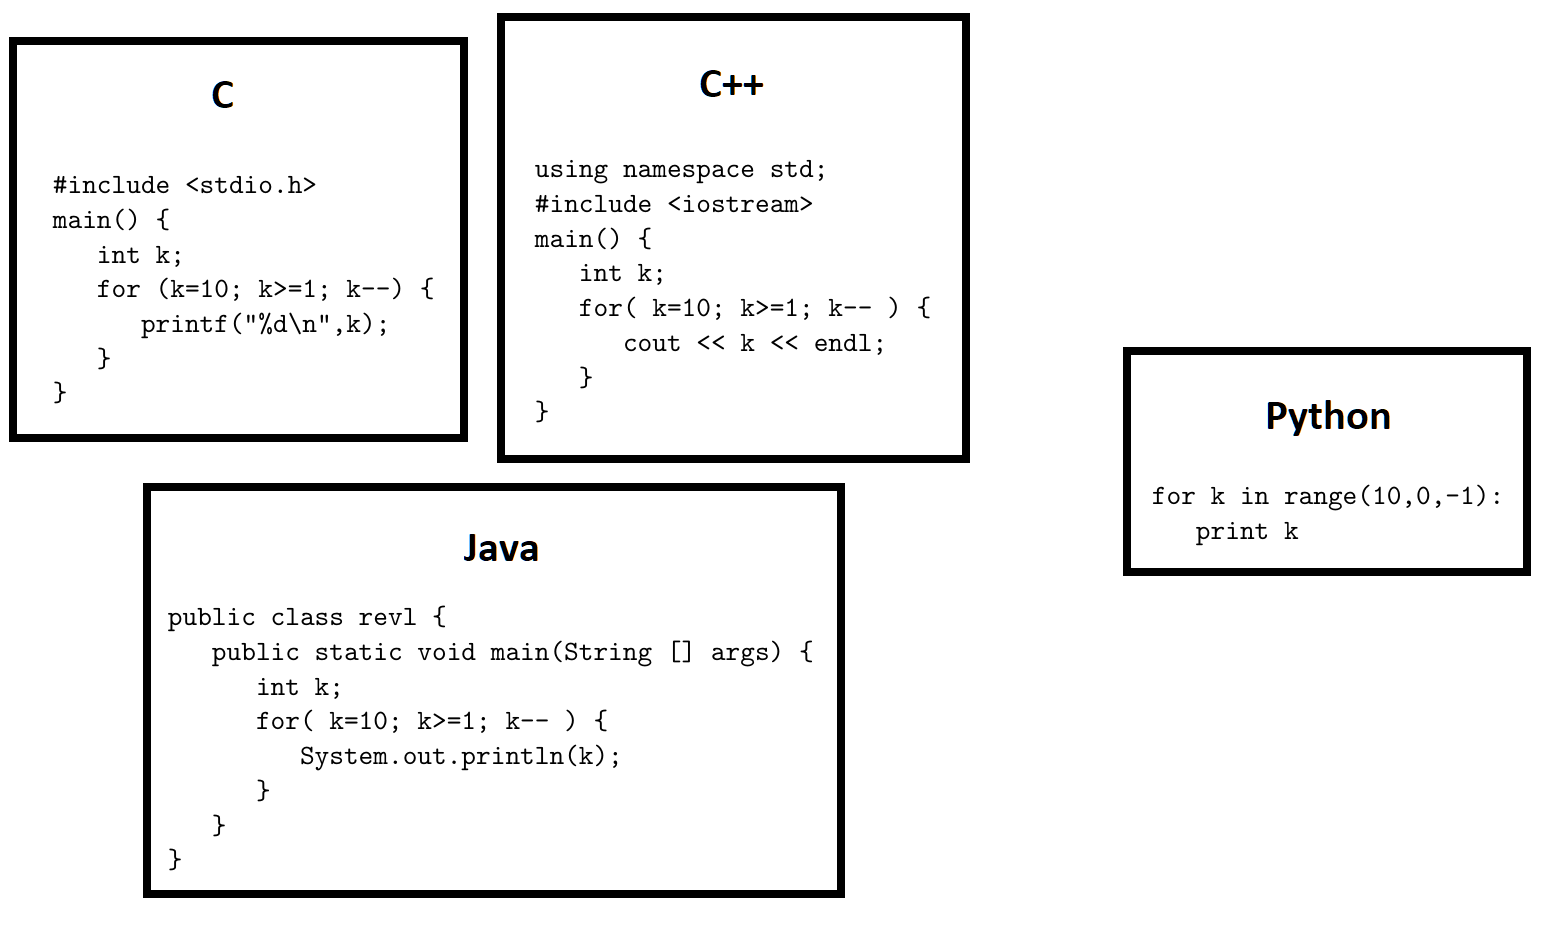
\includegraphics[width=0.9\linewidth]{SameLanguage}
				%\caption{Same program in 4 progamming languages}
			\end{figure}
		\endminipage\hfill
		
		\vspace{10pt}
		
		Moral of the story: \\
		Python is very easy to write and you can write in a single line what would take paragraphs in other languages
		
	\end{block}
	
\end{frame}

\begin{frame}	
	\frametitle{About Python}
	
	\begin{alertblock}{Some Python basics:}
		
		\vspace{8pt}
		
		\minipage{0.48\textwidth}
			Python programs are called \textbf{scripts} (standard convention for interpretted languages)
			\begin{figure}[ht]
				\centering
				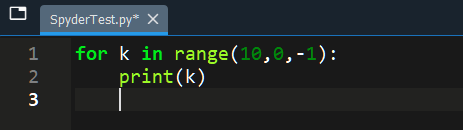
\includegraphics[width=0.9\linewidth]{ScriptExample}
				\caption{Example script from Spyder}
			\end{figure}
			
			\vspace{62pt}
			
		\endminipage\hfill
		\minipage{0.04\textwidth}
		\endminipage\hfill
		\minipage{0.48\textwidth}
			Python scripts are executed in a \textbf{shell} (command line interface, console, terminal)
			\begin{figure}[ht]
				\centering
				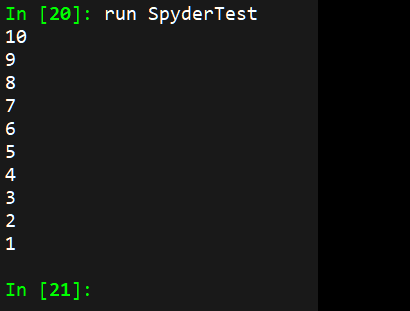
\includegraphics[width=0.9\linewidth]{ShellExample}
				\caption{Example console from Spyder}
			\end{figure}
		\endminipage\hfill
	\end{alertblock}
	
\end{frame}

\begin{frame}	
	\frametitle{About Python}
	
	\begin{alertblock}{Anaconda3 and Spyder:}
			\begin{itemize}
				\item In order to write a Python script, you need either a simple text editor or a more robust \textbf{IDE} (\emph{integrated development environment}). IDE's provide many additional features that simple text editors lack (debugging, syntax highliting, auto-completion, profiling, etc.).
				\item In order to run a Python script, you need to have some version of Python installed on your machine
			\end{itemize}
			
			\vspace{10pt}
		\minipage{0.48\textwidth}
			We will use Anaconda3, an open-source distribution of Python featuring most major scientific libraries and the Spyder IDE
		\endminipage\hfill
		\minipage{0.04\textwidth}
		\endminipage\hfill
		\minipage{0.48\textwidth}
			\begin{figure}[ht]
				\centering
				
\includegraphics[width=0.9\linewidth]{AnacondaLogo}
				%\caption{Example shell from Spyder}
			\end{figure}
		\endminipage\hfill
	\end{alertblock}
	
\end{frame}

\begin{frame}%[fragile]
	\frametitle{About Python}
	
	\vspace{-7pt}
	
	\begin{block}{Getting started with Spyder:}
			\begin{itemize}
				\item Install and launch Anaconda3 \href{https://www.anaconda.com/}{(LINK)}, Open Spyder
				\item Examine different panes: \\
						Editor, console, files, etc.
				\item Explore color themes: \\
						Tools $>$ Preferences $>$ Appearance
				\item Disable auto-completion features: \\
						Tools $>$ Preferences $>$ Editor $>$ Source Code \\
						Tools $>$ Preferences $>$ Completion and Linting
				\item Explore panes and layouts (under View tab)
			\end{itemize}
	\end{block}
	
\end{frame}

\begin{frame}%[fragile]
	\frametitle{About Python}
	
	\vspace{-7pt}
	
	\begin{block}{Getting started with Spyder:}
			\begin{itemize}
				\item Write and run (F5) simple script: \\
						\code{print(``Hello World'')}
				\item Use the file pane to navigate to an appropriate folder to save this script as HelloWorld.py
				\item While in that folder, you can also run the script by typing \\
				\code{run HelloWorld.py} in the console and pressing Enter
			\end{itemize}
	\end{block}
	
\end{frame}


%%%%%%%%%%
%%%%%%%%%%
\section{Objects and Operators}

\begin{frame}	
	\center{\Huge{Objects and Operators}}
\end{frame}

\begin{frame}%[fragile]
	\frametitle{Objects and Operators}
	
	\begin{alertblock}{Intro: objects and operators}
			Two of the main entities used in Python are
			\begin{itemize}
				\item \textbf{Objects}: pieces of data \\
						Ex: numbers, strings, lists, functions
				\item \textbf{Operators}: things which perform operations on objects \\
						Ex: number addition, string concatenation, comparison
			\end{itemize}
	\end{alertblock}
	
\end{frame}

\begin{frame}%[fragile]
	\frametitle{Objects and Operators}
	
	\begin{alertblock}{Data types:}
			Objects can be one of several fundamental data types (there are additional derived data types):
			\begin{itemize}
				\item \textbf{Integers} (\code{int}) \\
						Ex: 0, 1, -145350, $2^{20}$
				\item \textbf{Floating-point numbers} (\code{float}) \\
						Ex: 0.0, 1.0, 3.14159265, -2.4e4
				\item \textbf{Booleans} (\code{bool}) \\
						Ex: True, False
				\item \textbf{Strings} (\code{str}) \\
						Ex: 'a', 'qwerty', 'python is great'
			\end{itemize}
			(Note: you can use either single or double quotes for strings, just make sure both sides match)
	\end{alertblock}
	
\end{frame}

\begin{frame}%[fragile]
	\frametitle{Objects and Operators}
	
	\begin{alertblock}{Literals and variables:}
			\begin{itemize}
				\item \textbf{Literals} are constant values of some data type. They do not change and are not stored in memory. \\
						Ex: 100, 3.14e10, `KD9-3.7'
				\item \textbf{Variables} are labeled locations in memory which can store data \\
						Ex: \code{x, count, filename}
			\end{itemize}
			
			\vspace{10pt}
			
			\minipage{0.5\textwidth}
				\begin{itemize}
					\item To \emph{define} a variable, use the \textbf{assignment operator}: =
					\item You can change the value of variables
					\item You can even change their type
					\item You can't use a variable prior to defining it
				\end{itemize}
				
%				\vspace{10pt}
				
%				Having created \code{x}, we can print it and check its type
			\endminipage\hfill
			\minipage{0.5\textwidth}
				\begin{figure}[ht]
					\centering
					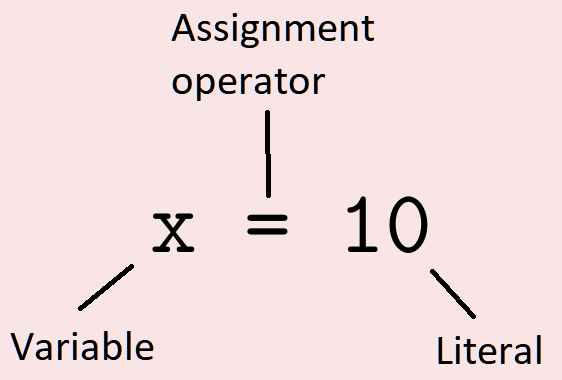
\includegraphics[width=0.9\linewidth]{Assignment}
					%\caption{Example shell from Spyder}
				\end{figure}
			\endminipage\hfill
	\end{alertblock}
	
\end{frame}

\begin{frame}%[fragile]
	\frametitle{Objects and Operators}
	
	\begin{block}{Notes on whitespace:}
			\begin{itemize}
				\item \code{x=10}, \code{x = 10}, \code{x\tab=10} are all interpreted the same way in Python
				\item You can also have as many blank lines as you want between non-blank lines
				\item Indentation is the only whitespace that matters (more on that later)
			\end{itemize}
	\end{block}
	
	\begin{block}{Rules for variable names:}
			\begin{itemize}
				\item Variables \emph{can} have upper/lower case characters, numbers, underscores
				\item Variables \emph{can't} have other symbols or start with numbers
				\item Variables \emph{can't} be pre-existing keywords: \code{for, in, while, if}
				\item A common convention for variable naming is \emph{camel case}: \code{isGreaterThanZero, stockPrice}
				\item Valid variable names: \code{\_x, test00, isNew, is\_new, zz45Z35ZZz}
				\item Invalid variable names: \code{is new, 0test, length\&OfString}
			\end{itemize}
	\end{block}
	
\end{frame}

\begin{frame}%[fragile]
	\frametitle{Objects and Operators}
	
	\begin{block}{Keywords:}
			Python also has a list of reserved keywords which CANNOT be used as variables:
			\begin{figure}[ht]
				\centering
				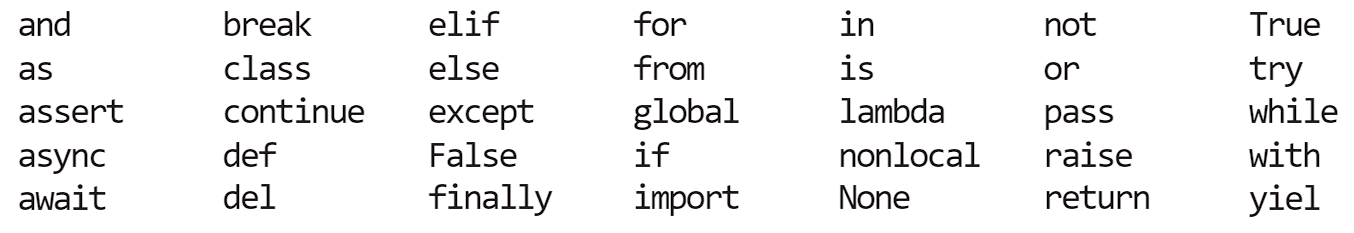
\includegraphics[width=0.9\linewidth]{Keywords}
				%\caption{Example shell from Spyder}
			\end{figure}
	\end{block}
	
	\begin{block}{Multiple assignment:}
			\begin{itemize}
				\item Python allows you to assign multiple variables in one line: \\
						Ex: \code{x, y = 1, 2}
				\item Useful when dealing with functions that return multiple outputs
			\end{itemize}
	\end{block}
\end{frame}

\begin{frame}%[fragile]
	\frametitle{Objects and Operators}
	
	\begin{alertblock}{Operators:}
			\textbf{Operators} take one or more objects and return new ones
			
			\vspace{10pt}
			
			Examples:
			\begin{itemize}
				\item Numeric: +, -, *, /, ** (exponent), \% (remainder) \\
						Note 1: numeric operators follow PEMDAS, group with parentheses \\
						Note 2: try mixing floats and ints in the same operation
				\item Boolean: == (comparison, checks for equality), != (not equal), $<, >, <=, >=,$ \code{not, and, or}
				\item String: + (concatenation), * (repetition), \code{[<int>]} (slicing/indexing, starts at 0, substring with colon), \code{in} (membership)
			\end{itemize}			
	\end{alertblock}
	
	\begin{alertblock}{Bonus: comments}
			Use the \# character to comment out a line
	\end{alertblock}
	
\end{frame}

\begin{frame}%[fragile]
	\frametitle{Objects and Operators}
	
	\begin{alertblock}{Expressions:}
			\textbf{Expressions} are formulas of a certain data type (the same as in math)
			
			\vspace{10pt}
			
			Examples:
			\begin{itemize}
				\item Numeric expressions return numeric values as their output \\
						(1.0+3*5)**0.5 \\
						\code{b}*\code{h/2}
				\item Boolean expressions return True/False as their output \\
						$1>2$ \\
						\code{x==1 and y==2}
				\item String expressions return strings as their output \\
						\code{'a'+'b'} \\
						\code{('a'+'b')}*\code{2}
			\end{itemize}			
	\end{alertblock}
	
\end{frame}

\begin{frame}%[fragile]
	\frametitle{Objects and Operators}
	
	\begin{alertblock}{Super brief intro to functions:}
			\begin{itemize}
				\item A \textbf{function} is a piece of code which takes some number of arguments as input and produces some sort of output
				\item Terminology: \\
						An argument is \textbf{passed} to a function \\
						The function \textbf{returns} the output \\
						(Note: some functions don't return anything, some don't need arguments)
%				\item If a function directly outputs some value which can be used or stored in a variable, we say that the function \emph{returns} that output
				\item Examples of functions: \\
						\code{print()} (displays text on console, does not return anything) \\
						\code{input()} (reads keyboard input from the console) \\
						\code{abs()} (returns absolute value of numeric input) \\
						\code{max()} (takes several numeric arguments, returns the maximum)
				\item Let's try passing different types to these functions
			\end{itemize}
	\end{alertblock}
	
\end{frame}

\begin{frame}%[fragile]
	\frametitle{Objects and Operators}
	
	\begin{alertblock}{Console/shell prompt notation:}
			\begin{itemize}
				\item The notation \shp denotes typing and running a command directly into a Python console
				\item The output of the command will be placed on the line below it without the notation
			\end{itemize}
	\end{alertblock}
	
	\begin{alertblock}{The \code{type()} function:}
			Use the Python function \code{type()} to discover what data type its input is:
			\begin{itemize}
				\item \shp \code{type(100)} \\ \code{int}
				\item \shp \code{type("red")} \\ \code{str}
			\end{itemize}
			NOTE: unless typing directly in the console, you must \code{print()} the output in order to see it in the console: \code{print(type(100))}
	\end{alertblock}
	
\end{frame}

\begin{frame}%[fragile]
	\frametitle{Objects and Operators}
	
	\begin{alertblock}{Casting data:}
			\textbf{Casting} is changing some data object from one type to another
			\begin{itemize}
				\item To cast, simply use the abbreviated name of the desired type as a function and pass your data to it
				\item Ex: \code{str(100)} will convert the integer 100 to the string `100'
				\item Ex: \code{int("100")} will convert the string `100' to the integer 100
				\item Ex: \code{int("abc")} will \emph{throw an error}
			\end{itemize}
			
%			\vspace{10pt}
			
			Casting floats and ints:
			\begin{itemize}
				\item When casting a float to an int, it always rounds down: \\
						\shp \code{int(1.7) \\ 1}
				\item When casting an int to a float, it appends a .0: \\
						\shp \code{float(1) \\ 1.0}
			\end{itemize}
	\end{alertblock}
	
\end{frame}

\begin{frame}%[fragile]
	\frametitle{Objects and Operators}
	
	\begin{block}{Weirdness with ints and floats:}
			Arguments to functions:
			\begin{itemize}
				\item Be aware that some functions on take ints as arguments, so passing floats will throw an error
				\item Passing an int to a function which takes floats is fine since it can simply cast it
			\end{itemize}
			
			\vspace{7pt}
			
			Integer division:
			\begin{itemize}
				\item In many languages (as well as previous versions of Python), the division of two integers would produce a truncated integer rather than a float
				\item As of Python 3 (the version we're using), integer division (//) and float division (/) have their own operators
				\item Keep in mind whether you need an integer or a float for specific applications (like string indexing)
			\end{itemize}
	\end{block}
	
\end{frame}


%%%%%%%%%%
%%%%%%%%%%
\section{Control Structures: Conditionals and Loops}

\begin{frame}	
	\center{\Huge{Control Structures: \\ Conditionals and Loops}}
\end{frame}

\begin{frame}%[fragile]
	\frametitle{Conditionals and Loops}
	
	\begin{alertblock}{Preview: conditionals and loops}
			Two critical programming constructs which control the flow of a program are:
			\begin{itemize}
				\item \textbf{Conditionals} (i.e., if statements) \\
				These cause the program to branch to one of several blocks of code based on whether different logical conditions are met
				\item \textbf{Loops} (i.e., for loops and while loops) \\
				These cause the program to repeat blocks of code until a certain condition is met
			\end{itemize}
	\end{alertblock}
	
\end{frame}

\begin{frame}%[fragile]
	\frametitle{Conditionals and Loops}
	
	\begin{alertblock}{Conditionals (if statements):}
		\minipage{0.5\textwidth}
			Prototypical if statement:
			
			\vspace{20pt}
			
			\code{if \emph{boolean expression}: \\
				\tab \emph{block of code} \\
				else: \\
				\tab \emph{block of code}}
			
			\vspace{20pt}
			
			(Note: italics in code snippets mean "some code goes here")
		\endminipage\hfill
		\minipage{0.5\textwidth}
			\begin{figure}[ht]
				\centering
				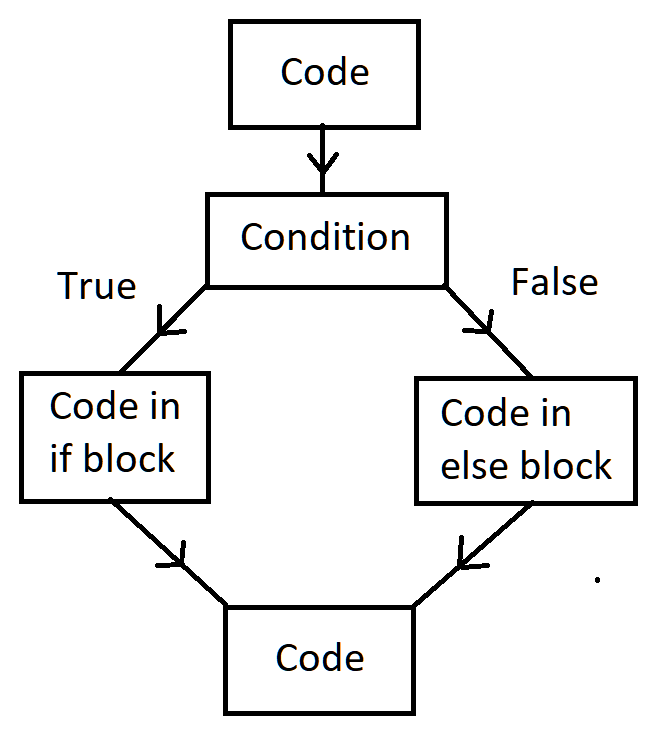
\includegraphics[width=0.9\linewidth]{ConditionalFlowchart}
				\caption{Flowchart for an if-else statement}
			\end{figure}
		\endminipage\hfill
	\end{alertblock}
	
\end{frame}

\begin{frame}%[fragile]
	\frametitle{Conditionals and Loops}
	
	\begin{block}{Conditionals (if-else statements):}
		\minipage{0.5\textwidth}
			\code{x = 11 \\
				\tab \\
				if x\%2 == 0: \\
				\tab print("x is even") \\
				else: \\
				\tab print("x is odd") \\
				\tab \\
				print("Done")}
				
				\vspace{10pt}
		\endminipage\hfill
		\minipage{0.5\textwidth}
			\begin{itemize}
				\item The Boolean expression should return either True or False
				\item Terminate the if/else lines with a colon (this signifies the start of a new code block)
				\item Indent all lines which should be part of each case's block
				\item To finish, revert one level of indenting
			\end{itemize}
		\endminipage\hfill
		
		\vspace{1pt}
		
		Indentation:
		\begin{itemize}
			\item Unlike most languages, \textbf{indentation is meaningful in Python}
			\item It is used to specify blocks of all kinds (if statements, loops, functions, classes, etc.)
		\end{itemize}
	\end{block}
	
\end{frame}

\begin{frame}%[fragile]
	\frametitle{Conditionals and Loops}
	
	\begin{block}{3 kinds of if statements:}
		You can have 1, 2, or more cases:
		
		\minipage{0.333\textwidth}
			\code{if \emph{bool exp}: \\
				\tab \emph{block of code}}
		\endminipage\hfill
		\minipage{0.333\textwidth}
			\code{if \emph{bool exp}: \\
				\tab \emph{block of code} \\
				else: \\
				\tab \emph{block of code}}
		\endminipage\hfill
		\minipage{0.333\textwidth}
			\code{if \emph{bool exp}: \\
				\tab \emph{block of code} \\
				elif \emph{bool exp}: \\
				\tab \emph{block of code} \\
				else: \\
				\tab \emph{block of code}}
		\endminipage\hfill
		
			\begin{itemize}
				\item \code{elif} is short for "else if"
				\item You can have as many \code{elif} case as you want
				\item You can have \code{elif} without the \code{else}
				\item Once the interpreter finds the correct case, the rest are skipped
			\end{itemize}
	\end{block}
	
\end{frame}

\begin{frame}%[fragile]
	\frametitle{Conditionals and Loops}
	
	\begin{block}{Nested if's:}
		
		\code{x = 11 \\
				\tab \\
				if x\%2 == 0: \\
				\tab if x\%3 == 0: \\
				\tab \tab print("x is divisible by 2 and 3") \\
				\tab else: \\
				\tab \tab print("x is divisible by 2, not 3") \\
				elif x\%3 == 0: \\
				\tab print("x is divisible by 3, not 2") \\
				else: \\
				\tab print("x isn't divisible by 2 or 3") \\
				\tab \\
				print("Done")}
		
	\end{block}
	
\end{frame}

\begin{frame}%[fragile]
	\frametitle{Conditionals and Loops}
	
	\begin{block}{Don't use separate if statements to account for all cases:}
		The code on the LEFT is better:
		
		\vspace{15pt}
		
		\minipage{0.5\textwidth}
			\code{if x\%2 == 0: \\
					\tab print("x is even") \\
					else: \\
					\tab print("x is odd")}
		\endminipage\hfill
		\minipage{0.5\textwidth}
			\code{if x\%2 == 0: \\
					\tab print("x is even") \\
					if x\%2 == 1: \\
					\tab print("x is odd")}
		\endminipage\hfill
		
		\vspace{15pt}
		
		Two issues:
		\begin{itemize}
			\item It evaluates an unnecessary Boolean expression, wasting computing time (though not much)
			\item If the conditions were more complex, it is possible it might miss additional cases (consider \code{x\%3})
		\end{itemize}
	\end{block}
	
\end{frame}

\begin{frame}%[fragile]
	\frametitle{Conditionals and Loops}
	
	\begin{block}{Using \#end comments:}
		\begin{itemize}
			\item Many languages require a keyword like \code{end} to finish if statements
			\item Python doesn't due to indentation, but adding them via comments can be a helpful visual aid
		\end{itemize}
		
		\vspace{5pt}
		
		\code{if x\%2 == 0: \\
				\tab if x\%3 == 0: \\
				\tab \tab print("x is divisible by 2 and 3") \\
				\tab else: \\
				\tab \tab print("x is divisible by 2, not 3") \\
				\tab \# end \\
				elif x\%3 == 0: \\
				\tab print("x is divisible by 3, not 2") \\
				else: \\
				\tab print("x isn't divisible by 2 or 3") \\
				\# end}
		
	\end{block}
	
\end{frame}

\begin{frame}%[fragile]
	\frametitle{Conditionals and Loops}
	
	\begin{exampleblock}{Exercise:}
		Write a Python script that will print the largest of three numbers (x,y,z)
	\end{exampleblock}
	
\end{frame}

\begin{frame}%[fragile]
	\frametitle{Conditionals and Loops}
	
	\begin{alertblock}{Loops:}
		\minipage{0.5\textwidth}
			Loops are coding constructs which repeatedly loop over (iterate) blocks of code until some condition is met
			
			\vspace{10pt}
			
			Two kinds of loops:
			\begin{itemize}
				\item \textbf{For loops} iterate over blocks a specified number of times and have an index variable that iterates through the number of iterations of the loop
				\item \textbf{While loops} iterate over blocks while a certain condition is true and then finish once the condition is false
			\end{itemize}
		\endminipage\hfill
		\minipage{0.5\textwidth}
			\begin{figure}[ht]
				\centering
				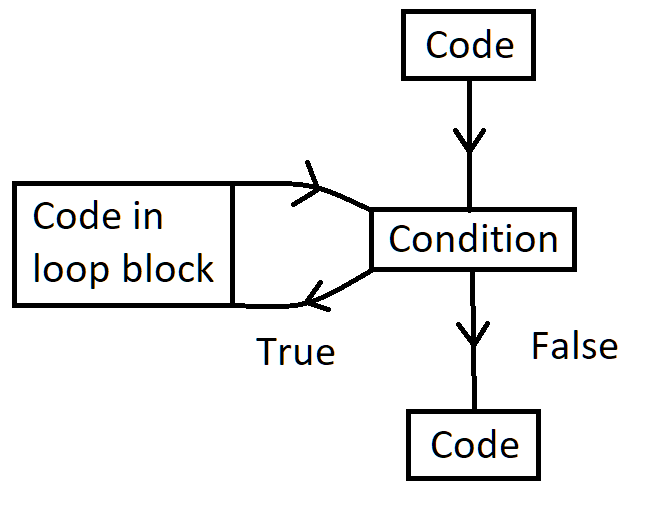
\includegraphics[width=0.9\linewidth]{LoopFlowchart}
				\caption{Flowchart for a while loop}
			\end{figure}
		\endminipage\hfill
	\end{alertblock}
	
\end{frame}

\begin{frame}%[fragile]
	\frametitle{Conditionals and Loops}
	
	\begin{block}{First for loop:}
		\minipage{0.5\textwidth}
			Here's a for loop which prints the integers from 0-9: \\
			
			\vspace{10pt}
			
			\code{
				for i in range(10): \\
				\tab print(i)}
			
			\vspace{20pt}
			
			How does range work:
			\begin{itemize}
				\item Start, end, increment
			\end{itemize}
		\endminipage\hfill
		\minipage{0.5\textwidth}
			\begin{itemize}
				\item Like with if's, use a colon to terminate the first line and indent the body of the block
				\item \code{range(10)} is a "list-like" object (it contains the sequence of values 0, 1, ..., 9)
				\item There are many list-like objects we can iterate over (we will learn about them later)
				\item For each iteration, \code{i} is set to a value in \code{range(10)} (via the keyword \code{in}) and can then be used in the body of the block
			\end{itemize}
		\endminipage\hfill
	\end{block}
	
\end{frame}

\begin{frame}%[fragile]
	\frametitle{Conditionals and Loops}
	
	\begin{block}{For loop examples:}
		\minipage{0.5\textwidth}
			Sum the integers 1-10: \\
			
			\vspace{10pt}
			
			\code{n = 10 \\
				total = 0 \\
				for i in range(1,n+1): \\
				\tab total = total + i}
		\endminipage\hfill
		\minipage{0.5\textwidth}
			Print even integers up to $10$ (inclusive): \\
			
			\vspace{10pt}
			
			\code{n = 10 \\
				for i in range(n+1): \\
				\tab if i\%2 == 0: \\
				\tab \tab print(i) }
		\endminipage\hfill
	\end{block}
	
\end{frame}

\begin{frame}%[fragile]
	\frametitle{Conditionals and Loops}
	
	\begin{block}{First while loop:}
		\minipage{0.5\textwidth}
			Here's a while loop which prints the integers from 0-9: \\
			
			\vspace{10pt}
			
			\code{i = 0 \\
				while i < 10: \\
				\tab print(i) \\
				\tab i += 1}
				
				\vspace{10pt}
		\endminipage\hfill
		\minipage{0.5\textwidth}
			\begin{itemize}
				\item Use a colon and indentation
				\item The loop keeps iterating until \code{i<10} is no longer True
				\item \code{i+=1} is Python shorthand for writing \code{i=i+1} (you can do this with any operator)
				\item \code{i+=1} increments the counter variable \code{i}
			\end{itemize}
		\endminipage\hfill
		
		\vspace{1pt}
		
		Infinite loops:
		\begin{itemize}
			\item Comment out the increment line, code loops forever
		\end{itemize}
	\end{block}
	
\end{frame}

\begin{frame}%[fragile]
	\frametitle{Conditionals and Loops}
	
	\begin{block}{While loop examples:}
		\minipage{0.5\textwidth}
			Print perfect squares less than \\ or equal to 100: \\
			
			\vspace{10pt}
			
			\code{i = 2 \\
				while i**2 < 100: \\
				\tab print(i**2) \\
				\tab i += 1}
				
%				\vspace{10pt}
		\endminipage\hfill
		\minipage{0.5\textwidth}
			
		\endminipage\hfill
	\end{block}
	
\end{frame}

\begin{frame}%[fragile]
	\frametitle{Conditionals and Loops}
	
	\begin{alertblock}{Continue and break:}
		\begin{itemize}
			\item Use \code{continue} to force a loop to skip the rest of the current iteration and jump to the next
			\item Use \code{break} to force a loop to skip the rest of the current iteration and end the loop
		\end{itemize}
	\end{alertblock}
	
\end{frame}

\begin{frame}%[fragile]
	\frametitle{Conditionals and Loops}
	
	\begin{alertblock}{Continue and break:}
		Print even integers up to 10:
		
		\vspace{10pt}
		
		\minipage{0.5\textwidth}
			\code{i = 0 \\
				while True: \\
				\tab if i\%2 != 0: \\
				\tab \tab i += 1 \\
				\tab \tab continue \\
				\tab else: \\
				\tab \tab print(i) \\
				\tab \# end \\
				\tab if i == 10: \\
				\tab \tab break \\
				\tab \# end \\
				\tab i += 1 \\
				\# end}
		\endminipage\hfill
		\minipage{0.5\textwidth}
			\code{
				for i in range(10+1):: \\
				\tab if i\%2 != 0: \\
				\tab \tab continue \\
				\tab else: \\
				\tab \tab print(i) \\
				\tab \# end \\
				\tab if i == 10: \\
				\tab \tab break \\
				\tab \# end \\
				\# end}
		\endminipage\hfill
	\end{alertblock}
	
\end{frame}





\begin{comment}


%%%%%%%%%%
%%%%%%%%%%
\section{Functions}

\begin{frame}	
	\center{\Huge{Functions}}
\end{frame}

\begin{frame}%[fragile]
	\frametitle{Functions}
	
	\begin{alertblock}{Review: functions}
		\begin{itemize}
			\item A \textbf{function} is a piece of code which takes zero or more arguments as input and produces some sort of output
			\item Terminology: \\
					An argument is \textbf{passed} to a function \\
					The function \textbf{returns} the output \\
			\item We've seen several of Python's standard functions: \code{print(), cast(), abs()}
			\item We can define our own functions
		\end{itemize}
	\end{alertblock}
	
\end{frame}

\begin{frame}%[fragile]
	\frametitle{Functions}
	
	\begin{alertblock}{Defn: functions}
		\begin{itemize}
			\item A \textbf{function} is a labeled block of code which runs when called
			\item A \textbf{block} is a specified piece of code that is utilized by various that is started by placing 
		\end{itemize}
		
		\vspace{10pt}
		
		\code{def myFunction(): \\
		\tab print("Hello from a function") \\
		\tab\\
		myFunction()}
		
		\vspace{10pt}
		
		Blocks:
		\begin{itemize}
			\item 
		\end{itemize}
	\end{alertblock}
	
\end{frame}


%%%%%%%%%%
%%%%%%%%%%
\section{Lists and Dictionaries}

\begin{frame}	
	\center{\Huge{Lists and Dictionaries}}
\end{frame}

\begin{frame}%[fragile]
	\frametitle{Lists and Dictionaries}
	
	\begin{alertblock}{Defn: scalar and non-scalar types}
		\begin{itemize}
			\item So far, most data types we have encountered have been a \textbf{scalar} type, i.e., it has no internal structure: \\
			Ex: ints, floats, and bools
			\item There are \textbf{non-scalar} types which DO have internal structure: \\
			Ex: strings, lists, dictionaries, tuples
		\end{itemize}
	\end{alertblock}
	
\end{frame}

\begin{frame}%[fragile]
	\frametitle{Lists and Dictionaries}
	
	\begin{alertblock}{Defn: lists}
		\begin{itemize}
			\item A \textbf{list} is an ordered set of data objects (called \textbf{entries} or \textbf{elements})
			\item They are represented and created using square brackets []
			\item They can have a mixture of different data types
			\item Examples: \\
					\code{[]} (the empty list) \\
					\code{[1,2,3,4,5]} \\
					\code{[`how', `now', `brown', `cow']} \\
					\code{[1,'x',True]}
			\item You can even have nested lists (lists within lists): \\
					\code{[ [1,2], [3,4] ]}
		\end{itemize}
	\end{alertblock}
	
\end{frame}

\begin{frame}%[fragile]
	\frametitle{Lists and Dictionaries}
	
	\begin{alertblock}{List indexing/slicing}
		\begin{itemize}
			\item Like strings, you can index lists using square brackets: \code{[$<$int$>$]} \\
					\code{\shp x = [`a','b','c','d','e','f'] \\
					\shp x[0] \\ `a' \\ \shp x[1:3] \\[1pt] [`b','c']}
			\item Indexing list literals can be confusing because the square brackets are being used in two ways in one line \\
			\code{\shp [1,2,3][1] \\ 2}
		\end{itemize}
	\end{alertblock}
	
\end{frame}

\begin{frame}%[fragile]
	\frametitle{Lists and Dictionaries}
	
	\begin{alertblock}{Common list functions: appending to lists}
		\begin{itemize}
			\item To append to a list, use either the + operator or the \code{.append()} function: \\
					\code{\shp x = [1,2,3] \\
					\shp x + [4] \\[1pt]
					[1,2,3,4] \\
					\shp x.append(4)} \\
					\shp print(x) \\[1pt]
					[1,2,3,4] \\
			\item The + way doesn't change \code{x} but does return the desired \code{[1,2,3,4]}; the \code{.append()} way doesn't return anything but changes the contents of \code{x}
		\end{itemize}
	\end{alertblock}
	
\end{frame}

\begin{frame}%[fragile]
	\frametitle{Lists and Dictionaries}
	
	\vspace{-4pt}
	
	\begin{alertblock}{Common list functions: len and sort}
		\begin{itemize}
			\item To find the length of a list, use \code{len()}: \\
			\code{\shp len([1,2,3]) \\
			3 }
			\item To sort a list, use \code{.sort()}: \\
			\code{\shp x = [6,2,8] \\
			\shp x.sort() \\
			\shp print(x) \\[1pt]
			[2,6,8]}
		\end{itemize}
	\end{alertblock}
	
	\vspace{-4pt}

	\begin{alertblock}{Common list functions: check membership}
		\begin{itemize}
			\item To check for membership in a list, use the \code{in} keyword: \\
			\code{\shp 1 in [1,2,3] \\
			True \\
			\shp 4 in [1,2,3] \\
			False}
		\end{itemize}
	\end{alertblock}
	
\end{frame}



\end{comment}


 
\end{document}








